% Capa
% ---
% Impressão da Capa
% ---
\begin{capa}
	\center
	UNIVERSIDADE FEDERAL DE ALAGOAS\\
	CENTRO DE TECNOLOGIA\\
	PROGRAMA DE PÓS GRADUAÇÃO EM ENGENHARIA CIVIL

	\vfill
	\MakeUppercase{\imprimirautor}

    \vfill
    \textbf{\imprimirtitulo}
    \vfill
    \vfill
    \imprimirlocal
    \par
    \imprimirdata

    \vspace*{1cm}
\end{capa}
% ---

% Folha de rosto (o * indica que haverá a ficha bibliográfica)
\imprimirfolhaderosto\

% Imprimir Ficha Catalográfica
% % ---
% Ficha Catalográfica
% ---
% Isto é um exemplo de Ficha Catalográfica, ou ``Dados internacionais de
% catalogação-na-publicação''. Você pode utilizar este modelo como referência.
% Porém, provavelmente a biblioteca da sua universidade lhe fornecerá um PDF
% com a ficha catalográfica definitiva após a defesa do trabalho. Quando estiver
% com o documento, salve-o como PDF no diretório do seu projeto e substitua todo
% o conteúdo de implementação deste arquivo pelo comando abaixo:
%
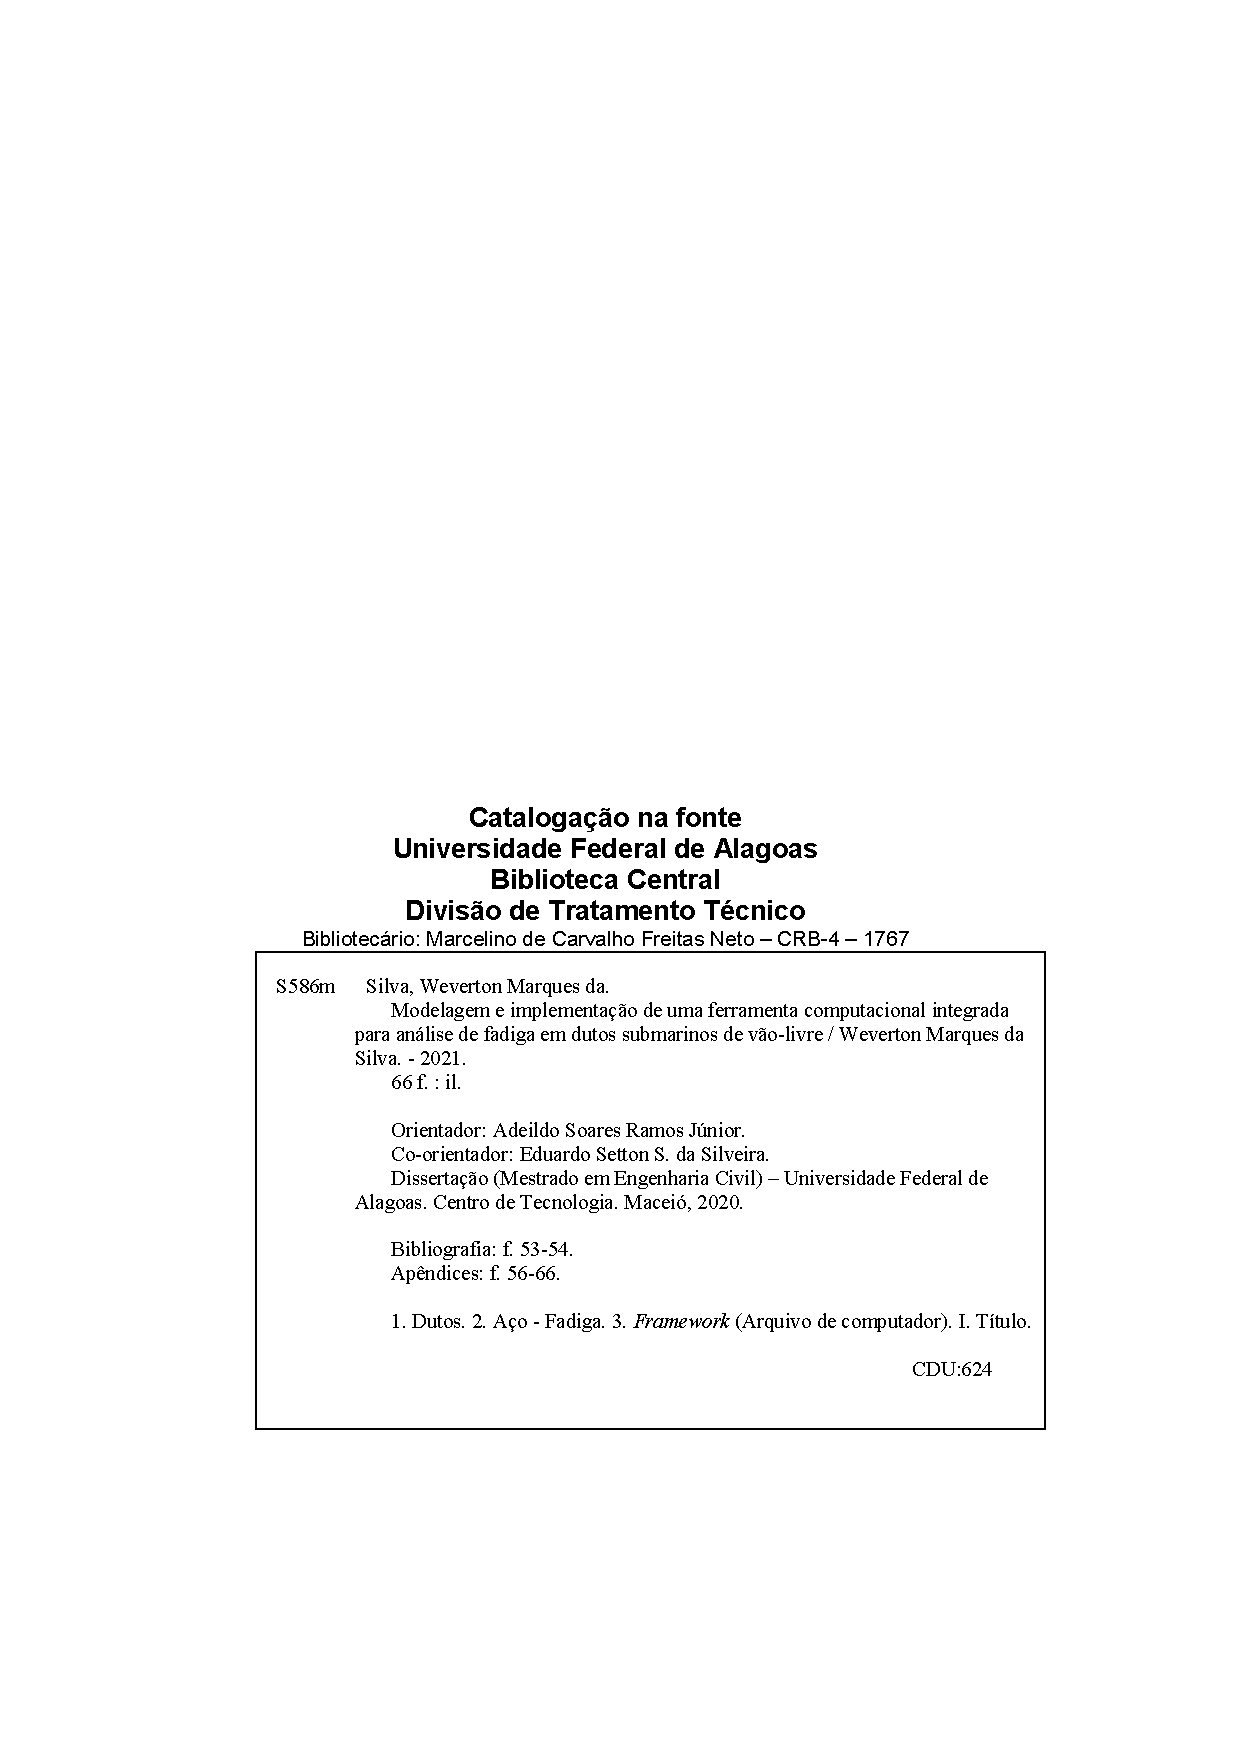
\includepdf{pretextual/ficha_catalografica.pdf}

% Inserir Folha de Aprovação
% ---
% Assinaturas
% ---
% Isto é um exemplo de Folha de aprovação, elemento obrigatório da NBR
% 14724/2011 (seção 4.2.1.3). Você pode utilizar este modelo até a aprovação
% do trabalho. Após isso, substitua todo o conteúdo deste arquivo por uma
% imagem da página assinada pela banca com o comando abaixo:
%
% \includepdf{folhadeaprovacao_final.pdf}
%
\begin{folhadeaprovacao}
	
\includepdf{pretextual/folha_de_aprovacao}
	% \begin{center}
	% 	\textbf{Folha de Aprovação}
	% 	\vfill

	% 	AUTOR: \MakeUppercase{\imprimirautor}

	% 	\vfill
	% 	\imprimirtitulo
	% 	\vfill

	% 	\hspace{.45\textwidth}
	% 	\begin{minipage}{.5\textwidth}
	% 		\imprimirpreambulo
	% 	\end{minipage}%
	% 	\vfill

	% 	Trabalho aprovado. \imprimirlocal, 28 de setembro de 2016:
	% \end{center}

	% \assinatura{\textbf{\imprimirorientador} \\ Orientador}
	% \assinatura{\textbf{\imprimircoorientador} \\ Co-Orientador}
	% \assinatura{\textbf{William Wagner Matos Lira} \\ Convidado 1}
	% \assinatura{\textbf{Leandro Melo de Sales} \\ Convidado 2}

\end{folhadeaprovacao}

% Dedicatória
% % ---
% Dedicatória
% ---
\begin{dedicatoria}
   \vspace*{\fill}
   \centering
   \noindent
   \textit{ Aos meus pais XXXXXXXX e YYYYYYY, \\ por sempre estarem comigo em todos os momentos.} \vspace*{\fill}
\end{dedicatoria}
% ---

% Agradecimentos
% % ---
% Agradecimentos
% ---
\begin{agradecimentos}

Aos meus familiares por todo apoio. Especialmente, ao meus irmão, Wagner, e a minha noiva, Jhulia, que estiveram sempre ao meu lado e me ajudaram a encontrar a disposição para seguir em frente.

Agradeço ao meu orientador e coorientador pelos direcionamentos e por acreditaram na importância dos frutos desse trabalho.

Ao Laboratório de Computação Científica e Visualização pela minha participação no projeto IntegriSpan. Especialmente aos meus amigos Emerson, Josué, Jéssica e Renato. Sem a ajuda e parceria inestimável deles este trabalho não seria possível.

Aos professores do Programa de Pós-Graduação em Engenharia Civil que, com os conhecimentos transmitidos nas disciplinas, me ajudaram a elaborar esse trabalho.

\end{agradecimentos}
%% ---

% Epígrafe
%% ---
% Epígrafe
% ---
\begin{epigrafe}
    \vspace*{\fill}
	\begin{flushright}
		\textit{``Seja curioso. Leia muito. Experimente coisas novas.\\ Eu acho que muito do que as pessoas chamam de inteligência\\apenas se resume a curiosidade.''\\ % chktex 38
		          (Aaron Swartz)}
	\end{flushright}
\end{epigrafe}
% ---

% Resumo e Abstract
% ---
% RESUMOS
% ---

% RESUMO em português
\setlength{\absparsep}{18pt} % ajusta o espaçamento dos parágrafos do resumo
\begin{resumo}
TODO.

 \textbf{Palavras-chaves}: TODO.
\end{resumo}

% ABSTRACT in english
\begin{resumo}[Abstract]
 \begin{otherlanguage*}{english}
   TODO.

   \vspace{\onelineskip}
 
   \noindent 
   \textbf{Keywords}: TODO.
 \end{otherlanguage*}
\end{resumo}

% Lista de ilustrações
\pdfbookmark[0]{\listfigurename}{lof}
\listoffigures*
\cleardoublepage

% Lista de tabelas
\pdfbookmark[0]{\listtablename}{lot}
\listoftables*
\cleardoublepage

% Lisa de listing (códigos)
% \providecommand{\listoflistings}{\listof{listing}{\listoflistingscaption}}
% \pdfbookmark[0]{\lstlistingname}{lol}
% \listoflistings
% \cleardoublepage

% Lista de abreviaturas e siglas
\begin{siglas}
  \item[MEF] Método dos Elementos Finitos
  \item[VIV] Vibração Induzida por Vórtice
\end{siglas}

% Lista de símbolos
%\begin{simbolos}
%  \item[$ \Gamma $] Letra grega Gama
%  \item[$ \Lambda $] Lambda
%  \item[$ \zeta $] Letra grega minúscula zeta
%  \item[$ \in $] Pertence
%\end{simbolos}

% Inserir o SUMÁRIO
\pdfbookmark[0]{\contentsname}{toc}
\settocdepth{section}
\tableofcontents*
\cleardoublepage